% -*- mode: latex-mode; TeX-engine: xetex; LaTeX-command-style: (("" "SOURCE_DATE_EPOCH=0 %(PDF)%(latex) --shell-escape %S%(PDFout)")); TeX-master: "../dissertation.tex"; -*-

\chapter{Raman Sideband Cooling}
\label{ch:rsc}

\section{Introduction}
(In order to achieve full quantum control on molecules, we need to control atoms first.)
(An example of such control)
(Motional degrees of freedom)
(PGC cools to ...)
(RSC to further cool.)
\todo{Define abbreviation RSC}
\todo{Maybe move some intro about large LD parameter here}

\section{Basic Theory}
\label{ch:rsc-basic-theory}

\begin{figure}
  \centering
  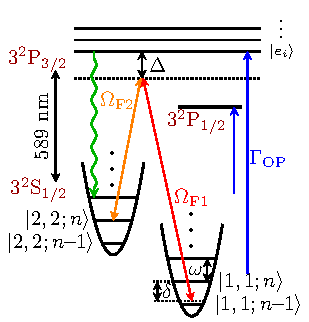
\includegraphics[width=8cm]{figures/na_rsc_schematics.pdf}
  \caption[Schematics of Raman sideband cooling for Sodium.]{
    Single Na atom Raman sideband cooling scheme.
    The Raman transitions couples $|2,2;n\rangle$ and $|1,1;n+\Delta n\rangle$
    through the intermediate states $|e_i\rangle$ in the $3^2P_{3/2}$ electronic states.
    The transitions have a one-photon detuning $\Delta_i\approx75$ GHz.
    Two-photon detuning, $\delta$, is defined relative to the $\Delta n=0$ carrier transition.
    For optical pumping, we use two $\sigma^+$ polarized transitions,
    one to pump the atom state out of $|1,1\rangle$ via $3^2P_{3/2}$
    and one to pump atoms out of $|2,1\rangle$ via $3^2P_{1/2}$
    to minimize heating of the $|2,2\rangle$ state.
    \label{fig:na-rsc-schematics}}
\end{figure}

The relevant energy diagram and the laser frequencies for RSC are shown in
Fig.~\ref{fig:na-rsc-schematics}.
We approximate the trapping potential using a harmonic oscillator.
Since this is a separable potential, we can use only the 1D motional state $|n\rangle$
and the result can be easily generalized to the full 3D system.

The cooling sequence consists of two types of pulses.
First, a Raman pulse drives the atom to a different hyperfine state while simultaneously
reduces the motional energy of the atom.
The optical pumping (OP) pulse afterwards then reset the hyperfine state of the atom
and reduce the entropy of the system.
This sequence is then repeated until the system reaches the ground motional state
where there is no more motional energy to be taken out of the system via the Raman pulse.
In this section, we will discuss the theory of each types of pulses individually.
We will cover how the pulses affect cooling performance in section \ref{ch:rsc-challenges}.

\subsection{Raman Transition}
\label{ch:rsc-basic-theory-raman}

As shown in Fig.~\ref{fig:na-rsc-schematics},
the cooling sequence starts with the sodium atom in the
$|s_1\rangle\equiv|2,2\rangle$ hyperfine state,
and a Raman transition is used to drive the atom to the $|s_2\rangle\equiv|1,1\rangle$ state,
where $|F,m_F\rangle$ denotes the $F$ and $m_F$ quantum number for the sodium atom.
The full Rabi frequency for such a transition is given by
\begin{align*}
  \Omega_R^0=&\sum_{i}\frac{\Omega_{1i}\Omega_{2i}^*}{2\Delta_i}
\end{align*}
where the sum is over all the coupled excited states,
$\Omega_{ai}\equiv\langle a|\mathbf{d}\cdot\mathbf{E}_a|e_i\rangle$ is the single photon
Rabi frequency between $|a\rangle$ and $|e_i\rangle$
and $\Delta_i$ is the single photon detuning from excited state $|e_i\rangle$.

In order to account for the motional degrees of freedom, we need to include the spatial
wavefunction of the atom and light into account.
As mentioned above, we approximate the atomic motional wavefunction by the harmonic oscillator
eigenstates $|n\rangle$. Coupling between states different $n$ states from the Raman transition
is allowed due to the recoil from the Raman lasers,
which corresponds to a spacial phase imprinting of $\ue^{\ui\mathbf{\Delta k}\cdot\mathbf{\hat x}}$
where $\mathbf{\Delta k}$ is the wavevector difference between the two Raman beams.
Using the creation ($\hat a^\dagger$) and annihilation ($\hat a$) operators and the relation
$\mathbf{\hat x}=\mathbf{x}_0\paren{\hat a+\hat a^\dagger}$ where $x_0=\sqrt{\hbar/2m\omega}$
is the harmonic oscillator length, the phase factor can be expressed as
$\ue^{\ui\eta^R\paren{\hat a+\hat a^\dagger}}$ where $\eta^R\equiv\mathbf{\Delta k}\cdot\mathbf{x}_0$
is the Lamb-Dicke parameter for the Raman transition \todo{\cite{}}.
The matrix element between motional state $|n\rangle$ and $|n'\rangle$ is therefore,
\[ M_{n,n'}=\langle n|\ue^{\ui\eta^R\paren{\hat a+\hat a^\dagger}}|n'\rangle \]
and the final Raman Rabi frequency between motional states $n$ and $n'$ is given by,
\[ \Omega_{R}^{n,n'}=M_{n,n'}\Omega_R^0 \]
For $n=n'$, this is called a carrier transition and the others are called sideband transitions.
If the final state is higher than the initial one, i.e. $n'>n$, it is a heating sideband.
Likewise, transitions with $n'<n$ are cooling sidebands.

A closed form result for $M_{n,n'}$ is given in \todo{\cite{}},
\[ M_{n,n'}=\ue^{\paren{\eta^R}^2/2}\sqrt{\frac{n_<!}{n_>!}}\paren{\eta^R}^{|n-n'|}L_{n_<}^{|n-n'|}\paren{\paren{\eta^R}^2} \]
where $n_<$ and $n_>$ are the lesser and greater, respectively, of $n$ and $n'$,
and $L_n^\alpha$ is the generalized Laguerre polynomial,
\[ L_n^\alpha(x)\equiv\sum_{m=0}^n(-1)^m\begin{pmatrix}n+\alpha\\n-m\end{pmatrix}\frac{x^m}{m!} \]

An important limit is the so-called Lamb-Dicke (LD) regime defined by $\paren{\eta^R}^2(2n+1)\ll 1$.
In this case, we can approximate the phase factor in leading order of $\eta^R$,
\[ \ue^{\ui\eta^R\paren{\hat a+\hat a^\dagger}}\approx1+\ui\eta^R\paren{\hat a+\hat a^\dagger} \]
and the matrix element
\[ M_{n,n'}\approx\delta_{n,n'}+\ui\eta^R\sqrt{n+1}\delta_{n+1,n'}+\ui\eta^R\sqrt{n}\delta_{n,n'+1} \]
the three terms corresponds to the carrier ($n'=n$),
the first order heating sideband ($n'=n+1$)
and the first order cooling sideband ($n'=n-1$) with corresponding strength
$1$, $\eta^R\sqrt{n+1}$ and $\eta^R\sqrt{n}$.
We can clearly see from this approximation that the coupling to other motional state
is stronger for a larger $\eta^R$ and higher motional quantum number $n$.
We will discuss this effect outside the LD regime and its implication
on the cooling performance in more detail in section \ref{ch:rsc-challenges}.

\subsection{Optical Pumping}
\label{ch:rsc-basic-theory-op}

Driving the system on a cooling sideband with Raman transition can reduce the
motional energy of the atom. However, this is a fully coherent process that does
not reduce the system entropy and is not really ``cooling'' the system
or achieving better control on the quantum state of the system.
Instead, quantum state control is achieved in the RSC via the OP pulse.
The initial hyperfine state $|2,2\rangle$ is a stretched state so it is the
state the system naturally ends up in when $\sigma^+$ light is applied.
However, if this is done using scattering from a $F=2$ to $F'=3$ transition,
the OP beam will allow continuous photon cycle
between the $|2,2\rangle$ and the $|3',3\rangle$ causing unnecessary motional heating during OP.
Therefore, the OP must be done on a $F=2$ to $F'=2$ transition.
Unfortunately, for Na, the corresponding transition from $3^2S_{1/2}$ to $3^2P_{3/2}$
that is used for the MOT is not useable due to the small energy difference of
$60 \mathrm{MHz}$ (or $6$ line widths) between the $F'=2$ and $F'=3$ states
\cite{steck_sodium_nodate}.
Instead, we must use the sodium $\mathrm{D1}$ line, i.e. $3^2S_{1/2}$ to $3^2P_{1/2}$ transition,
which lacks a $F'=3$ excited state.
The $\mathrm{D1}$ light with $\sigma^+$ polarization is only used to pump atoms from
$F=2$ states (in particular $|2,1\rangle$ which is populated during the OP process).
Since the goal of the OP pulse is to clear the atom population in all states but $|2,2\rangle$,
the photon cycling is not a concern for $F=1$ states and the $\mathrm{D2}$ line
is used for OP of $F=1$ states instead.
This also allow us to reuse the MOT light source and simplifies our setup.

\section{Raman Sideband Thermometry}

\todo{\cite{?}}From the discussion in section \ref{ch:rsc-basic-theory-raman},
we see that the strength of the sideband transition depends on the initial motional state
as well as the Lamb-Dicke parameter $\eta^R$ of the atom.
This dependency allows us to infer the motional state of the atom
by measuring the sideband height, i.e. the so-called sideband thermometry.

In particular, for atom with temperature $T$,
the probability for the atom to be in motional state $|n\rangle$ is,
\[ p_n=\frac{\ue^{-n\hbar\omega/k_BT}}{1-\ue^{-\hbar\omega/k_BT}} \]
for a Raman pulse with full Rabi frequency $\Omega_R^0$ and time $t$,
the peak height for the first order heating (+) and cooling (-) sidebands,
\begin{align*}
  h_\pm=&\sum_{n=0}^\infty p_n\sin^2\paren{\frac{\Omega_R^0t}{2}M_{n,n\pm1}}
\end{align*}
note that $p_{n+1}=p_n\ue^{-\hbar\omega/k_BT}$, $M_{n,n'}=M_{n',n}$ and $M_{n,-1}=0$, we have
\begin{align*}
  h_-=&\sum_{n=0}^\infty p_n\sin^2\paren{\frac{\Omega_R^0t}{2}M_{n,n-1}}\\
  =&\ue^{-\hbar\omega/k_BT}\sum_{n=1}^\infty p_{n-1}\sin^2\paren{\frac{\Omega_R^0t}{2}M_{n-1,n}}\\
  =&\ue^{-\hbar\omega/k_BT}h_+
\end{align*}
Therefore, if we measure the ratio of the cooling and heating sideband heights
$\alpha\equiv h_-/h_+$, we can calculate the temperature of the atom with
$\ue^{-\hbar\omega/k_BT}=\alpha$.
The corresponding ground state probability is,
\begin{align*}
  p_0=&\frac{1}{1-\ue^{-\hbar\omega/k_BT}}\\
  =&\frac{1}{1-\alpha}
\end{align*}
We will use this to experimentally characterize the performance of the cooling sequence
in the following sections.

\section{Setup}

\begin{figure}
  \centering
  \includegraphics[width=8cm]{figures/na_rsc_geometry.pdf}
  \caption[Beams and field geometry for Sodium Raman sideband cooling]{
    Geometry and polarizations of the Raman and optical pumping beams relative to the
    optical tweezer and bias magnetic field.
    Raman beams R1 and R4 address the radial $x$-mode.
    R1 and R2 address the radial $y$-mode.
    R3 and R4 address the axial $z$-mode, where the beams also couple to radial motion,
    but this coupling can be neglected when the atoms is cooled to the ground state of motion.
    \label{fig:na-rsc-geometry}}
\end{figure}

The geometry of all the beams and field involved is shown in Fig.~\ref{fig:na-rsc-geometry}.
In order to make the cooling more efficient and simplify the sideband thermometry,
we address the motion along the three principle axis of the tweezer using different pairs
of Raman beams.
We apply an external bias magnetic field of $8.8 \mathrm{G}$ parallel to the polarization
of the tweezer beam (and orthogonal to the tweezer beam propagation direction).
This makes the field orthogonal to the effective magnetic field of the tweezer,
which minimizes the vector light shifts~\cite{kaufman_cooling_2012,thompson_coherence_2013}.
Since the optical pumping beam requires $\sigma^+$ polarization,
it is setup to propagate parallel to the applied magnetic field.

\section{Cooling Performance and Challenge with Large Lamb-Dicke Parameter}
\label{ch:rsc-challenges}

\todo{some might belong to introduction of the chapter}
RSC is typically performed in the LD regime where the coupling
to other motional state is small.
Due to the light mass, short wavelength, limitted trap depth and high initial temperature
of the sodium atom however, we have to start our RSC sequence outside the LD regime.
This creates unique challenges to our experiment.
A detailed understanding of the cooling performance is required to understand
and overcome these challenges.

The simplest way to estimate the effectiveness of RSC
is by keeping track of the average energy of the atom during the cooling sequence.
For a typical RSC sequence in the LD regime, all the cooling are done on
the strongest first order cooling sideband.
The energy removed for atom driven in one Raman pulse is therefore, $\Delta E_-=\omega$.
In order to reinitialize the hyperfine state, the sodium atom needs to scatter on average
$2$ photons from the OP pulse which increases the average energy of the driven atom
by $\Delta E_+=4\omega_r$
\footnote{The factor of 4 comes from 2 absorbed photons and 2 reemitted photons.}
where $\omega_r\equiv \hbar k^2/2m$ is the recoil energy\cite{steck_sodium_nodate}
and $k$ is the OP light wave vector.
The heating to cooling ratio in one RSC pulse cycle is therefore,
\begin{align*}
  \frac{\Delta E_+}{\Delta E_-}=&\frac{2\hbar k^2}{m\omega}=4k^2x_0^2\\
  =&4\paren{\eta^{OP}}^2
\end{align*}
where $\eta^{OP}\equiv kx_0$ is the Lamb-Dicke parameter for OP.
Therefore, in order to achieve net cooling, we need $\paren{\eta^{OP}}^2<0.25$.
In 3D with cooling along multiple axis with different trapping frequency
(and therefore different $\eta^{OP}$), the $\paren{\eta^{OP}}^2$ in the requirement
is replaced by a weighted average of different axis depending on the frequency
each axis is cooled in the sequence.

\todo{change r to x in the plot to be consistent with text}
\begin{figure}
  \centering
  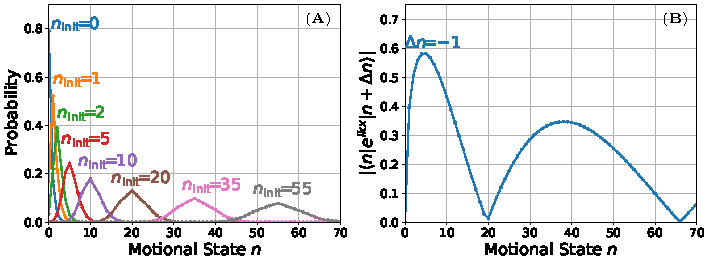
\includegraphics[width=\textwidth]{figures/na_rsc_challenges.pdf}
  \caption[Optical pumping motional-state redistribution and Raman coupling]{
    Optical pumping motional-state redistribution and Raman coupling for large LD parameters
    for the axial direction ($z$).
    The range plotted covers $95$\% of the initial thermal distribution.
    (A) Motional state distribution after one OP cycle for different initial states motion,
    $n_{\textrm{init}}$.
    Due to photon-recoil and the large LD parameter, $\eta^{\textrm{OP}}_z=0.55$,
    there is a high probability of $n$ changing.
    (B) Matrix elements for Raman transition on the first order cooling sideband
    deviate from $\sqrt{n}$ scaling with multiple minima.
    \label{fig:na-rsc-challenges}}
\end{figure}

In our experiment, the OP Lamb-Dicke parameters are
$\eta^{OP}_x, \eta^{OP}_y, \eta^{OP}_z = 0.25, 0.25, 0.55$.
Based on the metric above, any cooling sequences
that have fewer than $78\%$ cooling pulse for $z$ (axial) axis, which is generally the case,
should have a net cooling effect.
This, however, does not guarantee cooling into the ground motional state,
nor does it fully characterize the efficiency of the cooling sequence
since the averaging hides a few critical aspect of having a large Lamb-Dicke parameter.

One of the important effects can be seen in Fig.~\ref{fig:na-rsc-challenges}A showing
the motional state distribution after one OP cycle
for different initial motional states $n_{init}$.
Although the average heating is fixed at $4\omega_r$, independent of $n_{init}$,
the spread or the uncertainty of $n$ after the OP is significantly higher for high $n_{init}$.
This effect significantly increases the difficulty in controlling the state during the
RSC sequence. It can negatively impact the cooling performance and
may lead to increased loss during cooling due to atom escaping to higher motional states.

The other important effect is the dependency of matrix element $M_{n,n+1}$
on the motional level $n$.
While this dependency is not a new effect, since the $\sqrt{n}$ dependency
on the cooling sideband strength exist even in the LD regime
and must be taken into account with pulse time variation\todo{\cite{}}
to achieve efficient cooling, the high Lamb-Dicke parameter adds even more complications.
As shown in Fig.~\ref{fig:na-rsc-challenges}B, rather than a simple $\sqrt{n}$ dependency,
it is a non-monotonic function and more importantly has multiple minima, so-called ``dead-zone'',
within the range of motional states we are interested in.
The coupling strength for states in the dead-zones can be reduced by more than ten times
which can significant affect the efficiency of the cooling pulse
and even makes it virtually impossible to drive Raman transitions on atoms in these states
in order to cool them further.
A cooling sequence can therefore accumulate pupolations in the dead-zones
rather than the ground state.
Their small coupling strength also reduce their signal level during
Raman sideband spectroscopy making these states nearly invisible to sideband thermometry
which further complicates the optimization of the cooling sequence.

\section{Solution: High Order Sidebands}
\label{ch:rsc-solution-high-orders}

\todo{change r to x in the plot to be consistent with text}
\begin{figure}
  \centering
  \includegraphics[width=8cm]{figures/na_rsc_mele_raman.pdf}
  \caption[Raman coupling including high order sidebands]{
    Matrix elements for Raman transition including high order sidebands.
    During cooling, we utilize the fact that high motional states couple most effectively
    to sidebands with large $|\Delta n|$ in order to overcome the issue with
    variation and dead zone in the coupling strengths.
    \label{fig:na-rsc-mele-raman}}
\end{figure}

The main solution to the issues related to the large Lamb-Dicke parameter
is in fact the large Lamb-Dicke parameter itself.
The increased coupling to other motional state for large Lamb-Dicke parameter
and high motional states applies not only to $|\Delta n|=1$ but to higher $\Delta n$ as well.
Fig.~\ref{fig:na-rsc-mele-raman} shows the coupling to higher order cooling sidebands
which all have comparable strengths as the first order sidebands in different ranges
of motional states.

Because of this, it is now possible, and in some cases preferred, to apply Raman cooling pulse
on the higher order sidebands instead of only the first order one.
These pulses reduce more energy from the system per pulse which directly improves
the cooling to heating ratio and allows better control on the motional state
given the uncertainty after an OP pulse.
More importantly, depending on the motional level, there is always a sideband order
with significant coupling strength that can be used to cool it,
therefore completely removing the coupling dead-zones.
Moreover, by using each sideband orders only near their coupling maxima,
the coupling strength variation is also greatly reduced which removes
the need to vary the pulse times for all but the pulses on the first order sideband.

\section{Solution: Simulation Based Optimization}

\begin{figure}
  \centering
  \includegraphics[width=\textwidth]{figures/na_rsc_sequence.pdf}
  \caption[Simulation optimized Raman sideband cooling sequence for Sodium]{
    Schematic of the cooling pulse sequence. The tweezer is strobed at 3 MHz to
    reduce light shifts during optical pumping~\cite{hutzler_eliminating_2017}.
    Each cooling cycle consists of $8$ sideband pulses.
    The four axial pulses address two sideband orders.
    The two pulses in each radial direction either address $\Delta n=-2$ and $\Delta n=-1$
    or have different durations to drive $\Delta n=-1$,
    at the end of the cooling sequence when most of the population is below $n=3$.
    The Raman cooling and spectroscopy pulses have Blackman envelopes~\cite{kasevich_laser_1992}
    to reduce off-resonant coupling,
    while the measurement Rabi pulses in Fig.~\ref{fig:na-rsc-rabi-flop}
    have square envelopes to simplify analysis.
    \label{fig:na-rsc-sequence}}
\end{figure}

The change in cooling technique by including higher order sidebands, however,
does not remove the effect of coupling variation on the sideband thermometry.
If a non-thermal distribution of motional states is produced by the cooling sequence,
the ratio of the first order sideband height still cannot be trusted to calculate
the temperature or the ground state probability.
Including higher order sidebands in the sideband thermometry could in principle
give us enough information about the state distribution but doing
so for a non-thermal distribution is not easy or reliable.
We therefore use a Monte-Carlo simulation to guide our search
for the optimal sequence \todo{\cite{}}.\todo{More detail?}
Fig.~\ref{fig:na-rsc-sequence} demostrate the sequence from the simulation.
In particular, we find that alternating the cooling pulses between two
neighboring orders for the axial direction and $\Delta n=-2$ and $\Delta n=-1$
for the radial directions
eliminates the accumulation of population in motional states with small Raman coupling.
The simulation also confirms that setting the coupling strength of each sideband
to drive a Rabi $\pi$-pulse corresponding to the maximum matrix element motional state
(i.e. the maxima in Fig.~\ref{fig:na-rsc-mele-raman}) yields efficient cooling, initially,
as we expected from section \ref{ch:rsc-solution-high-orders}.
The efficiency of cooling on higher-order sidebands diminishes
as the atom approaches the ground state, so the final cycles utilize only
the $\Delta n=-1$ sideband while alternating between the three axes.

\section{Calibration}
(Sideband/carrier)\todo{Use scattering to calibrate intensity}
(Cold vs hot)

\section{Cooling Performance}
% The full sequence can be found in appendix \ref{appendex:rsc}.

\ref{fig:na-rsc-spectrum}
\ref{fig:na-rsc-rabi-flop}

\begin{figure}
  \centering
  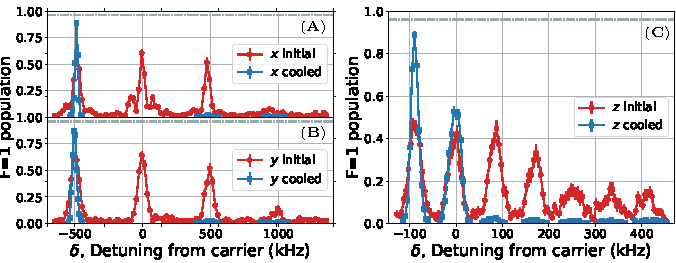
\includegraphics[width=\textwidth]{figures/na_rsc_spectrum.pdf}
  \caption[Raman sideband spectra before and after cooling]{
    Raman sideband spectra for (A) $x$, (B) $y$, (C) $z$ axis before (red circle)
    and after (blue square) applying Raman sideband cooling sequence.
    The height of the cooling sidebands (positive detuning)
    are strongly suppressed after cooling which suggests most of the atoms are cooled
    to the motional ground state in the trap.
    \label{fig:na-rsc-spectrum}}
\end{figure}

\begin{FPfigure}
  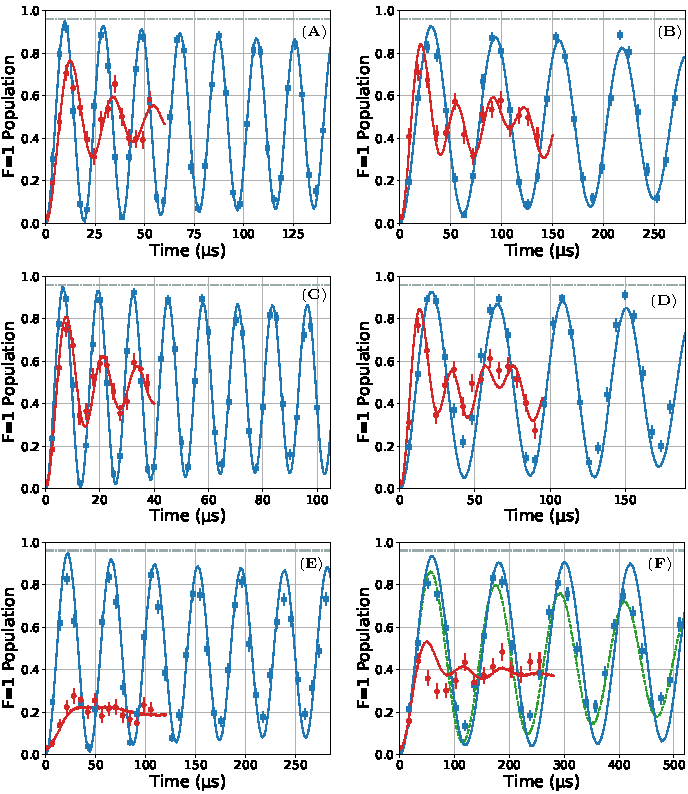
\includegraphics[width=\textwidth]{figures/na_rsc_rabi_flop.pdf}
  \caption[Rabi flopping on carriers and sidebands]{
    Rabi flopping on radial axis $x$ (A) carrier and (B) $\Delta n_x=1$ sideband,
    radial axis $y$ (C) carrier and (D) $\Delta n_x=1$ sideband,
    axial axis $z$ (E) carrier and (F) $\Delta n_x=1$ sideband,
    before (red circle) and after (blue square) Raman sideband cooling.

    Solid lines (both red and blue) in all plots are fits to a Rabi-flopping
    that includes a thermal distribution of motional states~\cite{meekhof_generation_1996}
    as well as off-resonant scattering from the Raman beams.

    The blue lines correspond to a ground state probability of (A-D) $98.1$\% along radial axis
    and (E-F) $95$\% along the axial axis after cooling.
    The red lines correspond to a thermal distribution of $80$ $\mu$K before RSC.
    The horizontal dashed lines in all the plots correspond to the $4\,\%$ probability
    of imaging loss.

    The green dashed line in (F) includes the additional decoherence due to
    a fluctuation of the hyperfine splitting of magnitude $3$ kHz.
    We see that the decoherence effect is strongest for the post-cooling data on
    the axial $\Delta n_z=1$ sideband where the Rabi frequency is the lowest.
    \label{fig:na-rsc-rabi-flop}}
\end{FPfigure}
\afterpage{\clearpage}
